\subsection{Lazo de corriente} \label{sec:lazoI}

Se realizó la modificación de los parámetros nombrados en la sección  REF 5.4 y se corroboró que el error no aparecía al cambiar el modo de funcionamiento del variador.
Para realizar la comunicación del microcontrolador con el variador de velocidad se decidió utilizar el modo de funcionamiento de entrada analógica de dos hilos (Ai1- señal + hilo común) ingresados por la bornera de la figura \ref{fig:born}. Este modo analógico podía ser configurado de 0-10V o 0-20mA a través del “jummper J3” (Figura \ref{fig:placals}).

Se optó por la utilización del lazo de corriente, este tiene ventajas sobre el lazo de tensión ya  que es más estable en largas distancias y más inmune a los ruidos eléctricos e interferencias electromagnéticas respecto al lazo de tensión. Normalmente, se utilizan lazos de corriente de 4-20mA para poder observar si hubiera fallas en el circuito, por lo que fue necesario adaptar la señal generada por el micorontrolador para seguir el estándar.



\begin{figure}[h]
	\centering
	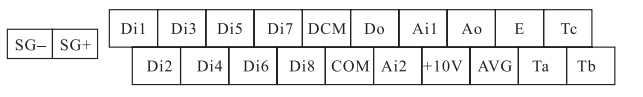
\includegraphics[width=0.7\linewidth]{imagenes/terminales.png}
	\caption{Terminales de control}
	\label{fig:born}
\end{figure}

\begin{figure}[htbp]
	\centering
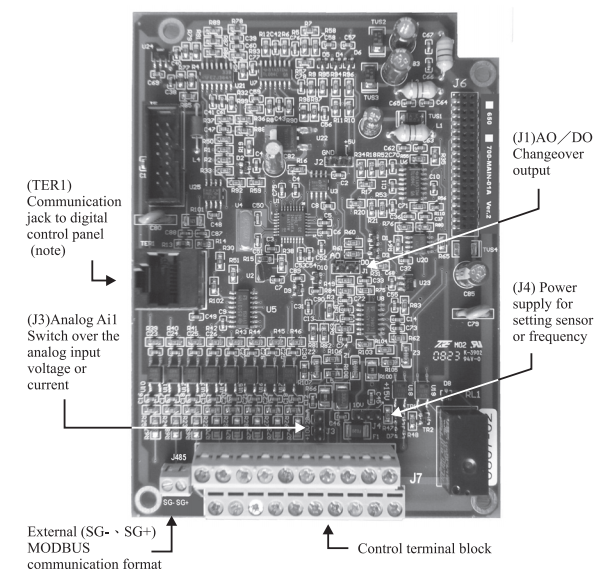
\includegraphics[width=0.7\linewidth]{imagenes/placa_ls}
\caption{Placa de control}
\label{fig:placals}
\end{figure}

La señal analógica para realizar el control del variador de velocidad fue generada por una señal PWM estipulada a través de la biblioteca \textit{TIMEROne} del microcontrolador. La instrucción \textit{Timer1.inizialize(period)} de la biblioteca Arduino inicializa el \textit{timer} con el valor de \textit{period}, este valor es el tiempo en el que se dispara el temporizador y en el caso de este proyecto es de 40 $u$s.

El otro comando que se utilizó fue \textit{Timer1.pwm(pin, duty)} que establece el número de
pin dónde sale la señal generada, en este caso pin 9 y \textit{duty} es un valor entre 0 y 1023 establecido por la programación, dónde 0 corresponde a 0mA (o 4mA). La salida del pin 9 corresponde a valores de tensión según el rango nombrado anteriormente, por lo que fue necesario realizar la transformación de esta señal a una señal de corriente utilizando un a “placa adaptadora de señal” (Figura \ref{fig:adapt}).

\begin{figure}[htbp]
	\centering
	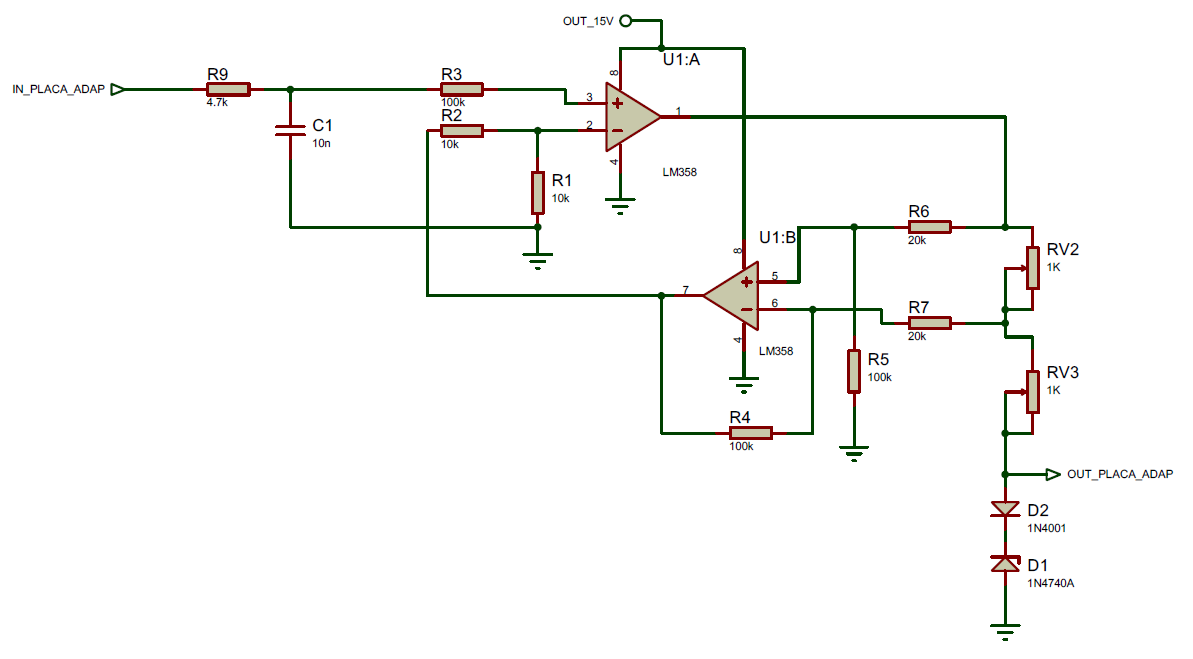
\includegraphics[scale=0.5]{adap_pl.png}
	\caption{Placa adaptadora de señal}
	\label{fig:adapt}
\end{figure}



\subsection{Estimación de la planta} \label{sec:estima}
    \subsubsection{Diagrama de trabajo}

Para realizar la estimación de la planta se muestra un diagrama de bloques del procedimiento que se siguió de forma resumida.

\begin{figure}[htb]
	\centering
	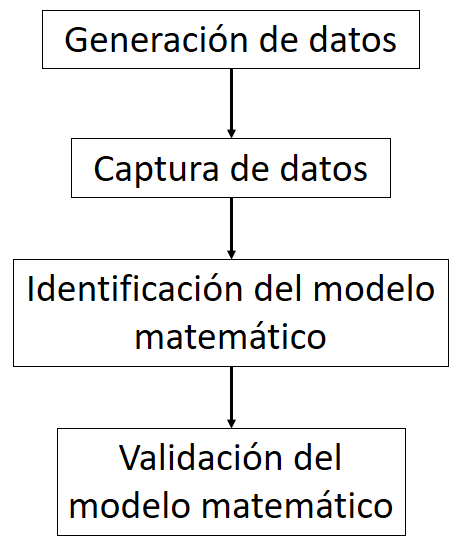
\includegraphics[scale=0.4]{planta_d.png}
	\captionof{figure}{Diagrama de bloques del procedimiento de modelado de la planta}
	\label{fig:planta_d}
\end{figure}

 \textbf{Generación de datos:} De acuerdo a diversas pruebas realizadas, se eligen las variables de mayor interés para analizarlas y asi poder enviar la información de forma eficaz.

 \textbf{Captura de datos:} A través del puerto serie y con Processing se realiza el almacenamiento de los datos de respuesta del sistema ante el estímulo de las señales de excitación. Posteriormente, el análisis de los datos y la generación de las gráficas correspondientes es realizado por medio de rutinas de código implementadas en Matlab.

 \textbf{Identificación del modelo matemático:} Se utilizaron varios métodos de identificación experimental, todos ellos analizados con la respuesta al escalón del sistema.

 \textbf{Validación del modelo matemático:} Una vez obtenida la mejor estimación, se efectuó una validación adicional a partir de la comparación de datos experimentales con los teóricos generados en simulaciones.






    \subsubsection{Método de estimación}

    Una vez que se determinó valores de ventana de filtro, velocidad de conmutación de PWM, tiempos de aceleración y desaceleración, etc. Se utilizó el modo de ingreso de señal por lazo de corriente al variador de velocidad. 
    
    La Figura \ref{fig:bloques} muestra un diagrama resumido de los pasos a realizar para tomar datos de la planta. Siendo G(s) el conjunto del túnel de viento, variador de velocidad y motor.
 
    \begin{center}
    	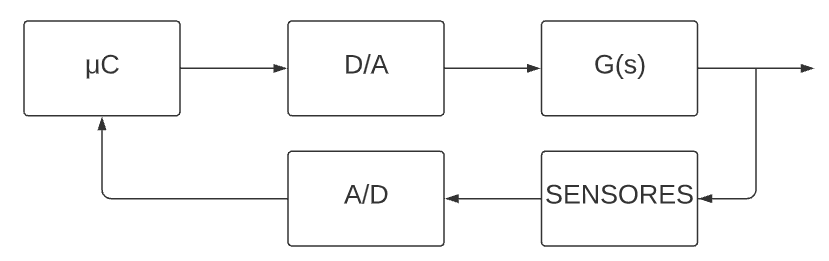
\includegraphics[scale=0.35]{bloques.png}
    	\captionof{figure}{Diagrama en bloques}
    	\label{fig:bloques}    
    \end{center}
    
    Para realizar la estimación de la planta se obtuvo y guardó tablas de datos con Processing, en las que se generó distintos escalones de entrada para la obtención varias mediciones. En la figura \ref{fig:est2} se observan los datos de dos columnas de las tablas anteriormente generadas.
    
    \begin{figure}[htb]
    	\centering
    	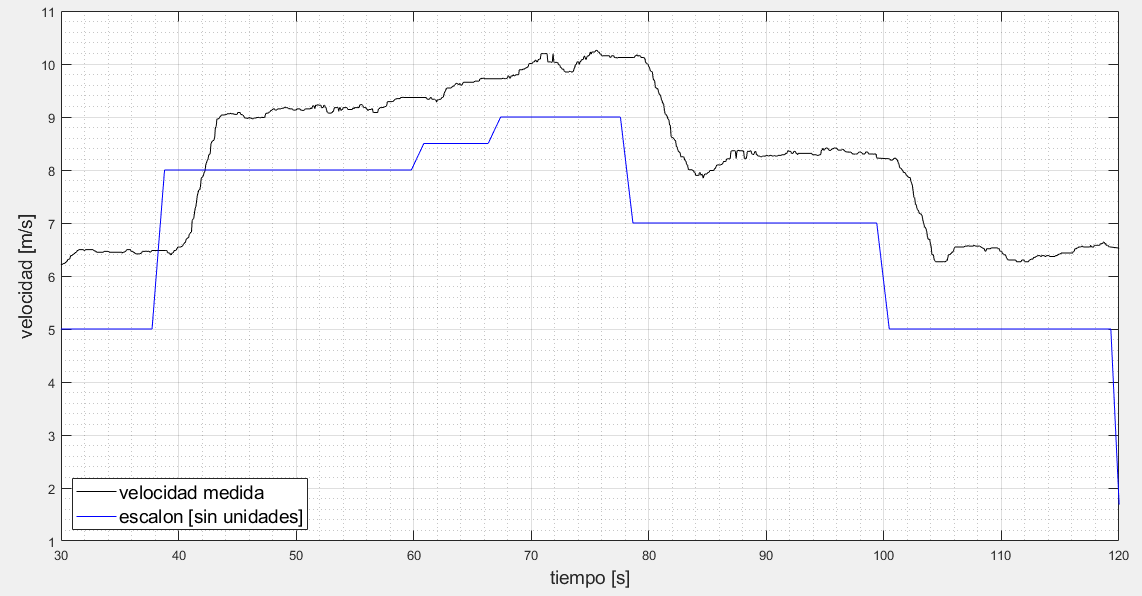
\includegraphics[scale=0.5]{estima.png} %pruba_1 del 0607
    	\captionof{figure}{Mediciones de velocidad a partir de distintos escalones dados}
    	\label{fig:est2}    
    \end{figure}
    
    Seguidamente, se procedió a generar un nuevo código de Matlab donde se cargaron los valores obtenidos de la figura (a) \ref{fig:pl2} para realizar la estimación de la planta a través de la comparación con la función de transferencia de un sistema de \textit{"2° orden con retardo"} \cite{pomares2011sistemas}.
    
    \begin{figure}[htbp]
    	\centering
    	\subfigure[Parámetros respuesta 2° orden]{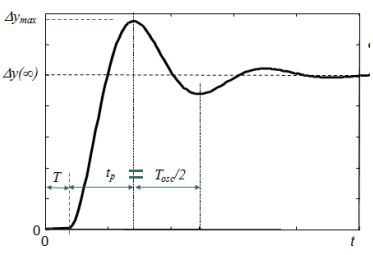
\includegraphics[width=70mm]{parametros_seg.png}}
    	\subfigure[Estimación de parámetros]{\includegraphics[width=80mm]{planta_seg1.png}} 
    	\caption{Estimación de planta} \label{fig:pl2}
    \end{figure}

 \begin{equation}
 	G(s)=\frac{k\omega_n^2}{s^2+2\xi\omega_ns+\omega_n^2}\ast e^{-T.s}
 \end{equation}

Sobreoscilación: 
\begin{equation}
	\delta\;=\;\frac{\triangle y_{max}-\triangle y\left(\infty\right)}{\triangle y\left(\infty\right)}=\;e\;^{-\frac{\xi\pi}{\sqrt{1-\xi^2}}}\;\;\;\rightarrow\;Para\;obtener\;\xi
\end{equation}

Tiempo de pico: 
\begin{equation}
t_p\;=\;\frac{T_{osc}}2\;=\;\frac\pi{\omega_n\sqrt{1-\xi^2}}\;\;\rightarrow\;Para\;obtener\;\omega_n
\end{equation}

    
    Con ayuda del código y ajustes manuales se llegó a una función de transferencia de segundo orden:
    
    \begin{equation}
    	\frac{Y(s)}{U(s)}=\frac{0,02483}{s^2+1,846s+1,535}
    \end{equation}
   
    Esta función de transferencia esta realizada para una entrada que va desde 0 a 1023. Que es el límite mínimo y máximo para determinar el ancho de pulso de la señal PWM del microcontrolador.
    
    Para corroborar la elección de la planta se realizó en \textit{Simulink} la respuesta del sistema a los mismos escalones experimentales. Seguidamente en el gráfico se dispuso la respuesta experimental en conjunto con la simulación (Figura \ref{fig:estim2} y Figura \ref{fig:estim3}).
    
    \begin{figure}[H]
    	\centering
    	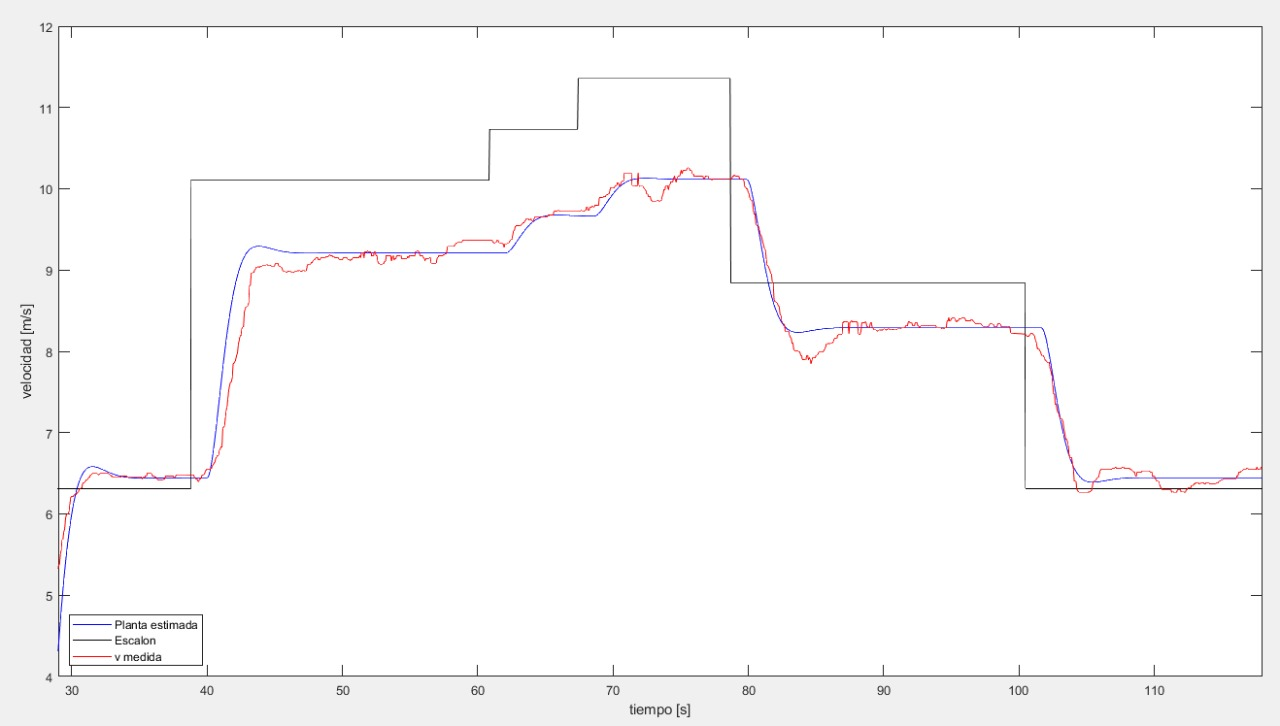
\includegraphics[scale=0.35]{estim2.jpeg}
    	\captionof{figure}{Corroboración de estimación de la planta. Ejemplo 1}
    	\label{fig:estim2}
    \end{figure}

\begin{figure}[H]
	\centering
	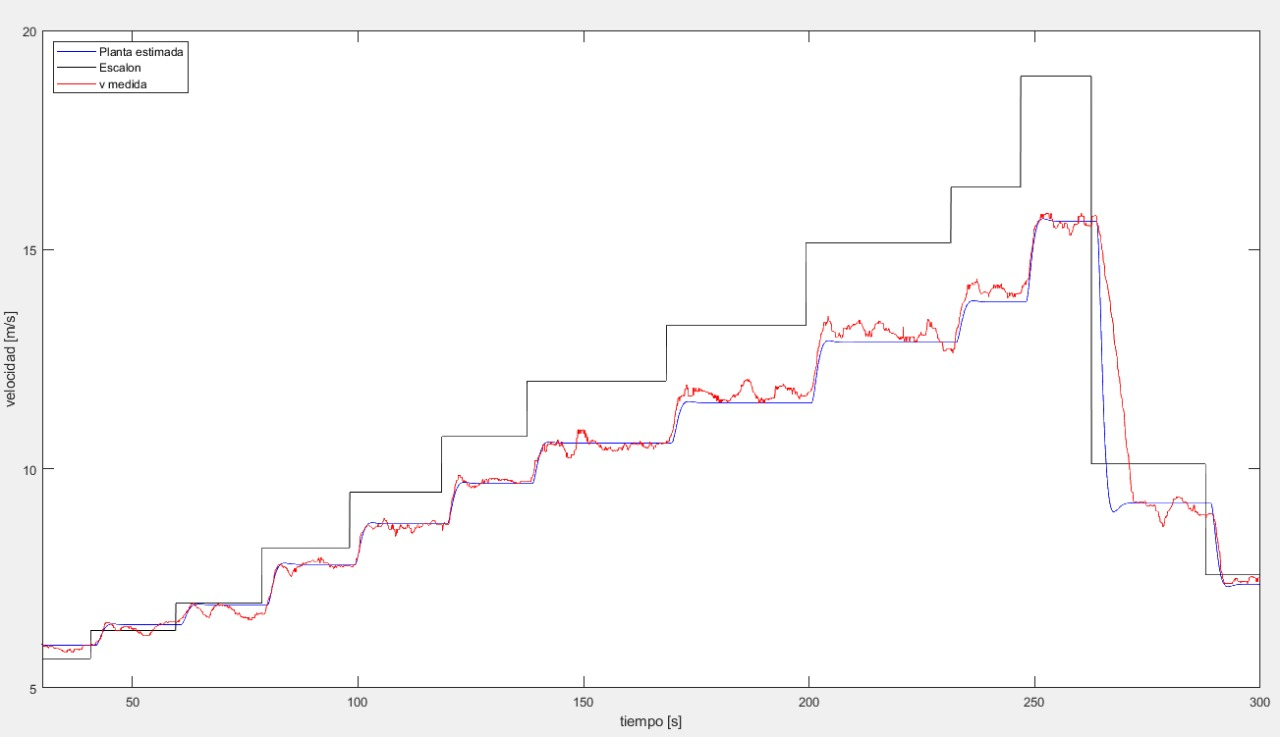
\includegraphics[scale=0.35]{estim3.jpeg}
	\captionof{figure}{Corroboración de estimación de la planta. Ejemplo 2}
	\label{fig:estim3}
\end{figure}
       
    \subsection{Control}
    Para el cálculo en primera instancia del controlador PID se utilizó la herramienta de \textit{Matlab}, y a partir de los primeros valores se realizaron pequeñas modificaciones todas en el formato PI (proporcional - integrador) hasta obtener varios tipos de respuesta.
    Con los distintos valores de PI se realizaron pruebas en el Túnel del viento con escalones de velocidad de referencia de 6 - 7,5 - 8,5 - 7,5 - 7 - 6 m/s, haciendo un total de 5 pruebas para los mismos estímulos de entrada. 
   
    \begin{figure}[H]
    	\centering
    	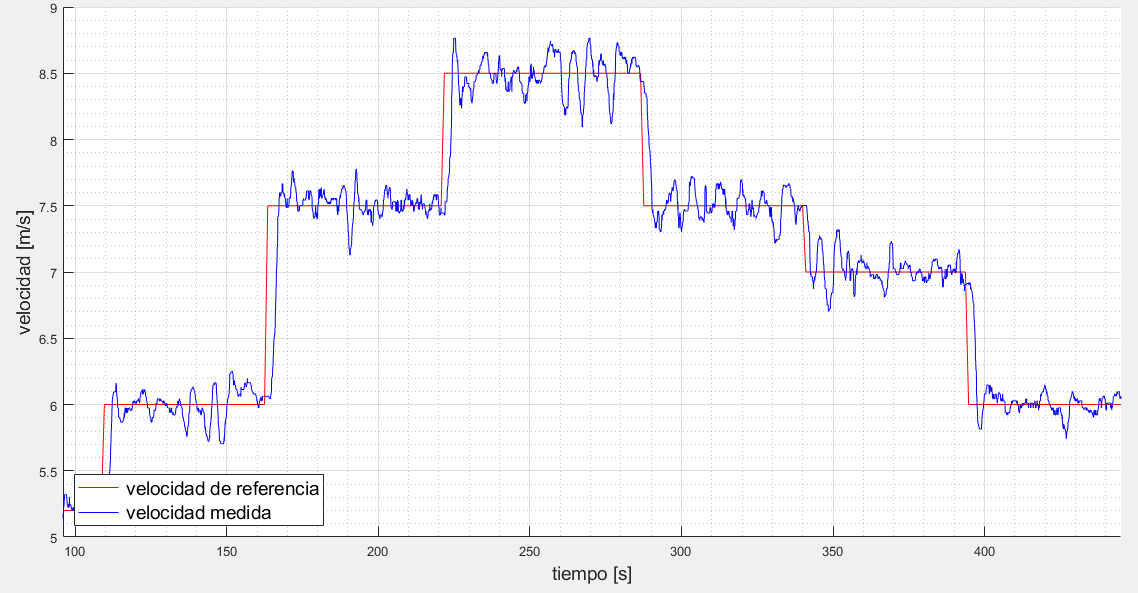
\includegraphics[scale=0.5]{pruebapid.png}
    	\captionof{figure}{Ejemplo de prueba realizada}
    	\label{fig:PI3}
    \end{figure}
    
    Los valores de cada configuración PI se muestran en la tabla siguiente
    \begin{table}[H]
    	\centering
    	\begin{tabular}{r|r|r|r|r|r|r|}
    		\cline{2-7}
    		\multicolumn{1}{l|}{} & \multicolumn{1}{c|}{\textbf{PI anterior}} & \multicolumn{1}{c|}{\textbf{Prueba3}} & \multicolumn{1}{c|}{\textbf{Prueba4}} & \multicolumn{1}{c|}{\textbf{Prueba5}} & \multicolumn{1}{c|}{\textbf{Prueba6}} & \multicolumn{1}{c|}{\textbf{Prueba7}} \\ \hline
    		\multicolumn{1}{|r|}{\textbf{P=}} & 0.225 & 0.0699 & 0.244 & 0.5451 & 0.6846 & 0.3286 \\ \hline
    		\multicolumn{1}{|r|}{\textbf{I=}} & 0.326 & 0.2035 & 0.2756 & 0.3599 & 0.4183 & 0.3107 \\ \hline
    	\end{tabular}
    \caption{Valores de PID's}
    \end{table}
    
    Al visualizar las respuestas obtenidas por las diferentes configuraciones se puede realizar la comparacion para un escalon en donde la velocidad sube (figura \ref{fig:pisubuda}) y otro donde la velocidad baja (figura \ref{fig:pibajada}).
    
    \begin{figure}[H]
    	\centering
    	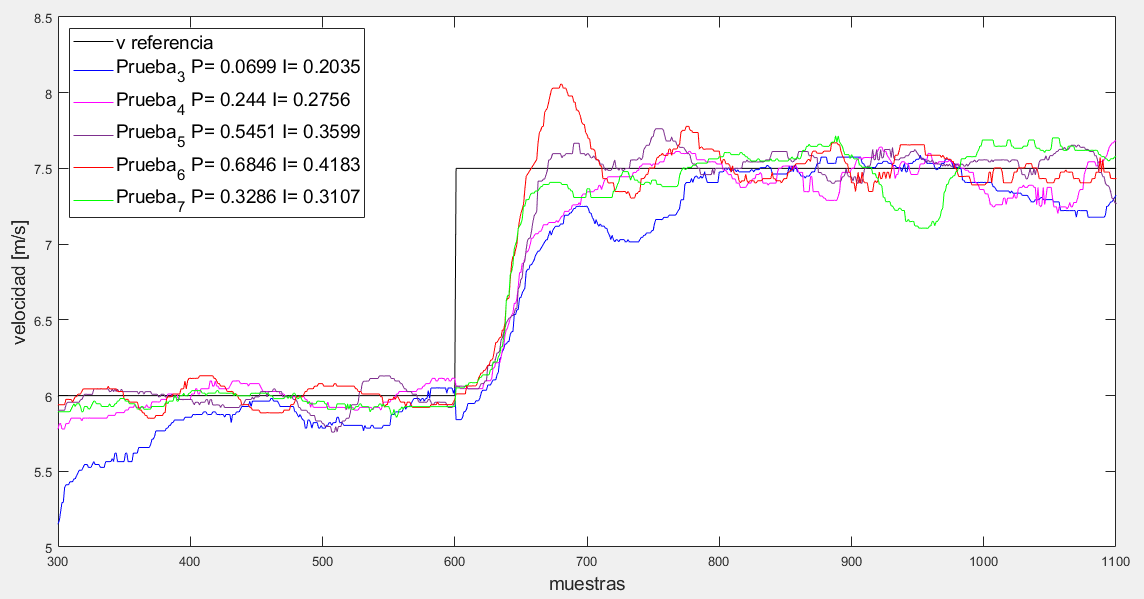
\includegraphics[scale=0.5]{pisubida.png}
    	\captionof{figure}{Comparación de PI, escalon de subida}
    	\label{fig:pisubuda}
    \end{figure}
    
    \begin{figure}[H]
    	\centering
    	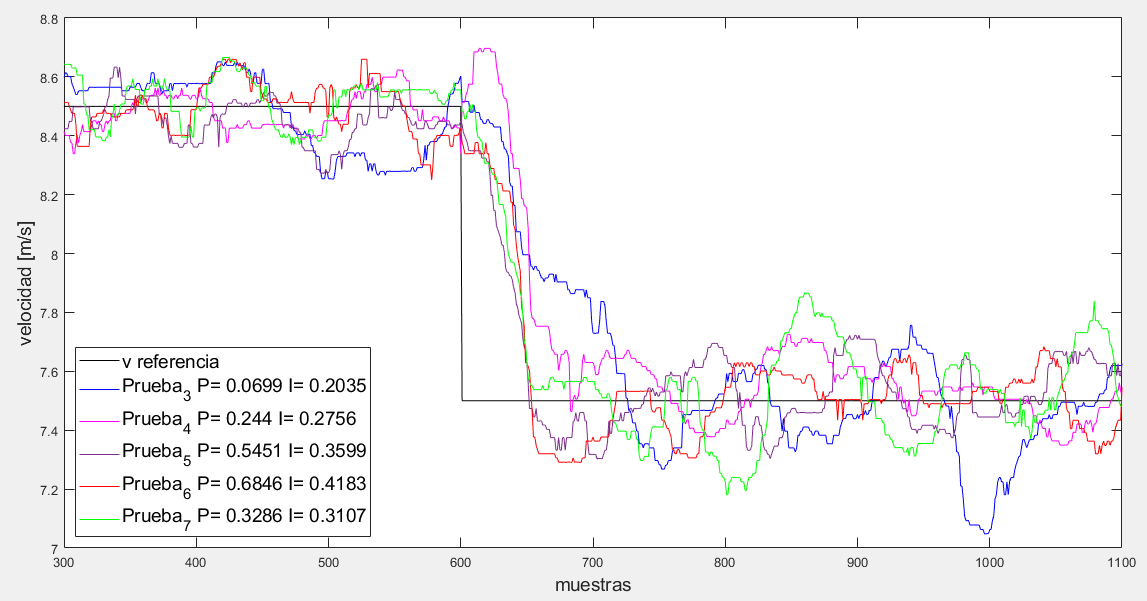
\includegraphics[scale=0.5]{pibajada.png}
    	\captionof{figure}{Comparación de PI, escalon de bajada}
    	\label{fig:pibajada}
    \end{figure}
    
    
    En la figura \ref{fig:mix} se pueden observar el sistema que genera mayor sobrepico, un sistema con una respuesta mas lenta, y un sistema con respuesta intermedia. 
    \begin{figure}[h!]
    	\centering
    	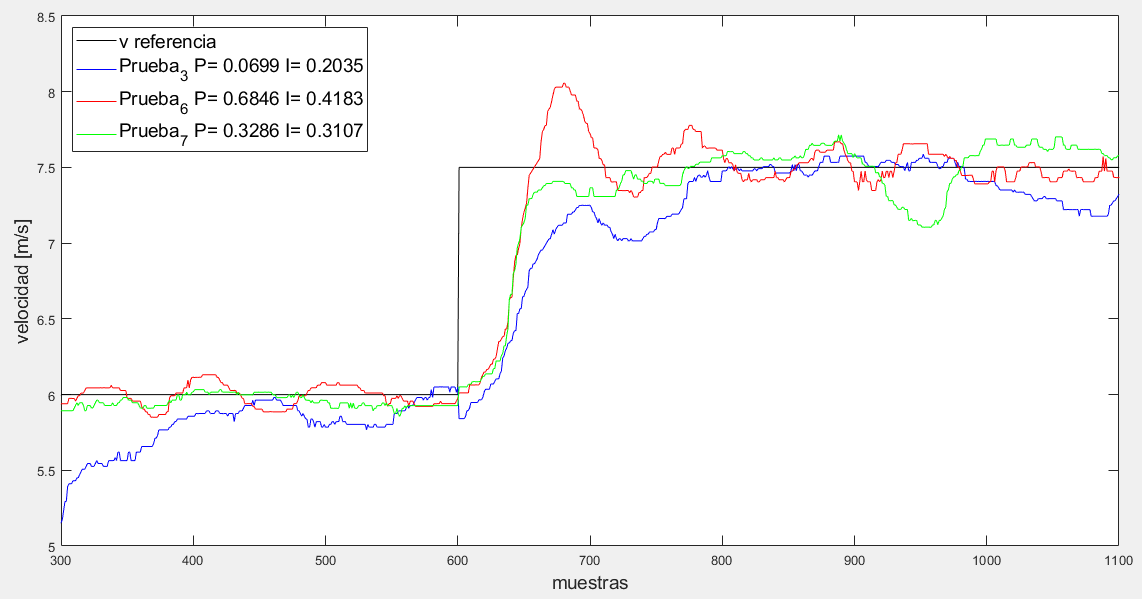
\includegraphics[scale=0.5]{mix.png}
    	\captionof{figure}{Comparación 3 sistemas PI}
    	\label{fig:mix}
    \end{figure}
    
    \newpage